%%% This LaTeX source document can be used as the basis for your technical
%%% report. Intentionally stripped and simplified
%%% and commands should be adjusted for your particular paper - title, 
%%% author, citations, equations, etc.
% % Citations/references are in report.bib 

\documentclass[conference]{acmsiggraph}
\usepackage{lipsum}

\TOGonlineid{45678}
\TOGvolume{0}
\TOGnumber{0}
\TOGarticleDOI{1111111.2222222}
\TOGprojectURL{}
\TOGvideoURL{}
\TOGdataURL{}
\TOGcodeURL{}

\title{Performance analysis of Real Time Physically Simulated Scenes \\
	   Design Document}

\author{Sam Serrels\\\ 40082367@napier.ac.uk \\
Edinburgh Napier University\\
Physics-Based Animation (SET09119)}
\pdfauthor{Sam Serrels}

\keywords{Multi-platform Physics, Optimisation, GPU, Cell, PS3}

\begin{document}

\teaser{
   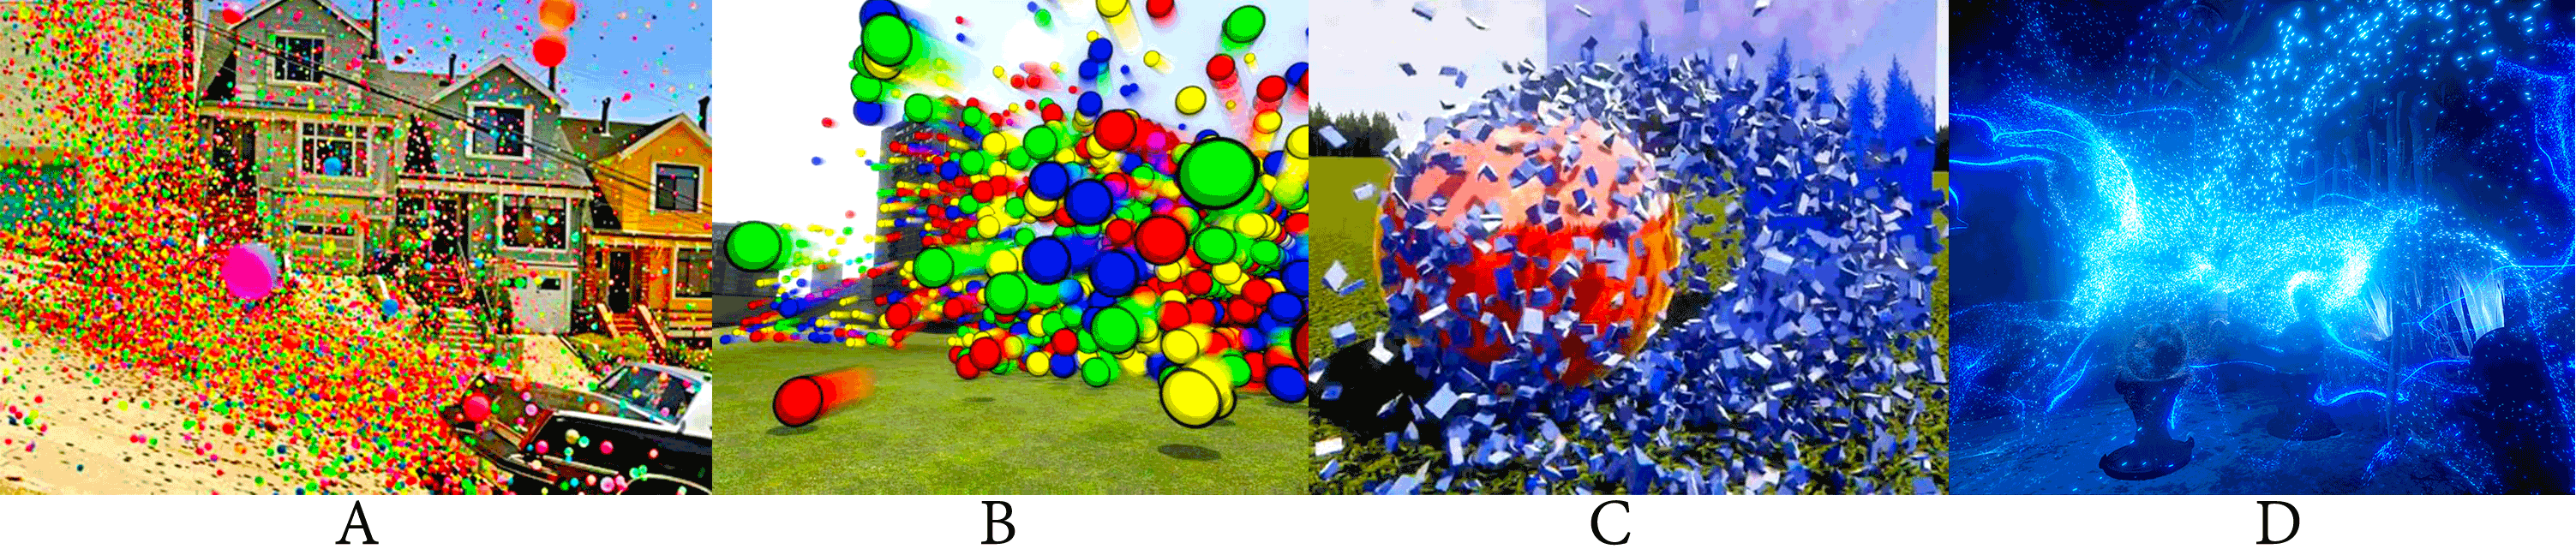
\includegraphics[height=1.5in]{images/sampleteaser}
   \caption{(a) soft bodies, (b) particles, (c) inverse kinematics, (e) fur shells, and (f) position-based dynamics for cloth effects.}
 }

\maketitle

\begin{abstract}
Realistic Real time physics simulation is highly sought after in interactive applications, especially games. Achieving high-accuracy while maintaining performance in often resource restricted environments(I.E a games console) requires the highest level of optimisations and often results in a trade-off with simulation speed against Accuracy. This project attempts to record and analyse the performance of various optimisations on a simulated scene. This will be taken further by applying the project to various different processing architectures. The scene that will be simulated is a large set of Bouncy balls, travelling down a hill.
\end{abstract}

\keywordlist
%\copyrightspace

\section{Introduction}

\paragraph{Physics Engines}
Large and complex video games tend to use 3rd party physics solutions, this vastly cuts down on the project development man-hours, and the maintenance thereafter. Third party physics solutions have the benefit of being battle tested out in the wild beforehand, so internal reliability is usually a given. A further benefit is that being developed solely for the purpose of being a "a good physics engine" by people who are usually experts in the field, large optimisations are already implemented. The problems arise in the implementation, the coupling of a physics engine and the existing codebase. While they are usually well coded, they are not tailor made to each game. 

\paragraph{Optimising for Physics Engines}
Trying to regain performance from an external physics engine can be a hard task, diving into the source code requires expert knowledge of the inner-workings of the whole system. A common path is to shape the design of the game code to conform better to the demands of the physics engine and hope that the internal optimisations  will be sufficient. Often enough, they are not.

\paragraph{Shipping on consoles}
Video games consoles have vastly varying hardware capabilities and architecture, writing robust code that is performant on all of them is a rarely possible. Code has to be re-designed for each system. The simple truth: more code = more problems, means that throwing a large complex physics engine that you have no knowledge of the inter-working of into the mix, is a recipe for bad performance and bad code. However some physics systems do have separate versions for different architectures, assuming the interface is unchanged, games can swap in different libraries at compile-time. A further extension on to this would be to abstract all the physics so many different libraries can be plugged in.

\paragraph{Project Aims}
This project will attempt to create a physics solution that will run on various systems, along with a game engine with an appropriate interface to swap in other existing physics solutions. This will allow for fair comparisons and benchmarking of the physics solution created by this project.

\paragraph{Project Application}
The systems created in the project will be used to simulate a demo scene, picked to be processing intensive. The scene will be a large set of bouncy balls, bouncing down a sloped street. This will result in plenty of collisions, a large amount of data needing transferred every frame, and something interesting to watch. The inspiration for this came from a Tv advert \cite{advert} where a similar thing was filmed in reality, with real bouncy balls and a real street.

\paragraph{Why is it hard}
\lipsum[32]

\paragraph{Why hasn't it been done before}
\lipsum[32]

\section{Related Work}

Refer to literature on the particular physics-based animation effect you want to synthesize (e.g., published articles, books, conference proceedings, web articles) provide a comprehensive review - and use the correct citation format, e.g., \cite{Sako00}.

Related work should finish with a summary paragraph - emphasising the crucial similarities or differences between existing methods presented in the literature.  For example: (1) you might want to modify the technique to run on the GPU; (2) or you combine different techniques from different authors; (3) or you are simplifying the algorithm to make it run faster.

\section{Overview}
Brief overview of the core principles and mechanism behind your effect.  This should be reflected in your final implementation, so consider what you will actually be implementing. What components make up the effect and how are they connected.


\section{Simulation}

How does your simulation work and what are the reasons it is important.  This is a decisive section to put together as it will help you in the rest of your physics-based animation development.

\begin{itemize}
\item{Physics-Based Animation Description}
Provide a more detailed description of how the simulation functions.
\item{Formal Elements}
Description of your simulation using the formal elements.  You should include the following sections.
\item{Interactive}
Describe the interactive pattern you are aiming for .
\item{Objectives}
What are the objectives of the simulation?  You may have one overall objective and some sub-objectives.
\item{Procedures}
What are the actions performed in the simulation.  Are there any specific technical workings?
\item{Rules}
What test cases have you defined to demonstrate the effectiveness of your technique?  Define a list of simple tests - both showing the good and the bad parts of your approach.
\item{Resources}
What are the resources within the solution?  Is it procedural?  Does it require artist intervention?  Is the solution scalable?  e.g., large and small scenes?
\item{Boundaries}
What are the boundaries of the technique?  This will probably be based on experiments - the technique might only fit specific situations (e.g., outside/inside/small high detail situations or crowds of low-level detail).
\item{Outcome}
What is the outcome?  Explain any possible issues?  Complexity? Computational power? Remember, relate this back to your investigations, related work, and experience - what have other people said?  Do you agree with them?
\end{itemize}

\section{Description}

\begin{itemize}
\item {Screen Mock-Ups \& Preliminary Screenshots}
Provide any screen mock-up of how your animation will look or preliminary screenshots.  You can use whatever method you see fit to create the mock-up.  Your mock-up doesn't have to be exactly how your simulation will look, and you can use in place graphics.  Explain principles and concepts to the reader - so you can explain your idea.
\item {Dynamic}
In this section you should describe any user interactive controls for customizing or changing the simulation - to effect the outcomes of the effect (e.g., adding external forces, numbers of objects, gravity)
\item {Control Mechanism}
Describe the control principles.  What controller mechanism have you gone for (i.e., random or from scripts)?  
\item {Rules}
Reflect upon the rules defined in the formal elements, and how these may affect the controls of the simulation.  Also consider any relationships between physical objects which might have an influence on the controls.
\item {Modes and Other Features}
Does your effect support multiple modes?  Are there any other features (e.g. novel control mechanisms) which need to be taken into account?
\item {Test Scenes}
Does your simulation have different scenes (2D, 3D, different complexity, real-time, off-line)?  If so, then design a variety of simple test cases to show the situations and demonstrate the viability of your technique.
\item {Flowchart}
Create an overview flowchart - and explain the interaction of the different components.  For example, do you update the forces, then move forwards, then draw....
\end{itemize}

\section{Technical Specification}

In this section, you should put together some of the technical details of your simulation.  This will help when developing your physics-based simulation later.

\begin{itemize}
\item {Technical Analysis} This section analyses the technical requirements of your simulation.  The goal here is to describe the main software development tasks, the risks involved, and any external libraries you are using.
\item {Major Software Development Tasks} What are the major pieces of development to make the software work?  Identify the main tasks from the simulation design, particularly items you feel will be difficult to implement.  List these here so you can approach these tasks individually.
\item {Risks} What are the risks in your development?  Consider which pieces of functionality will be difficult to implement, and what are the options if you cannot achieve them.
\item {External Libraries} Are you using any external libraries or resources to implement your simulation?  If you are using any libraries outside the ones developed in the practical sessions, these will need to be described here.
\end{itemize}


Equations should be numbered and in the correct format, e.g., Equation \ref{eq:myequation} below:

\begin{equation} \label{eq:myequation}
 \sum_{j=1}^{z} j = \frac{z(z+1)}{2}
\end{equation}


\section{Conclusion}
The report should finish with a summary to give a brief overview of what the reader should remember most.  What was most important?


% \section*{Acknowledgements}


\bibliographystyle{acmsiggraph}
\bibliography{report}

\end{document}

